\clearpage
% \setcounter{page}{1}
\maketitlesupplementary

\setcounter{section}{0}
\setcounter{figure}{0}
\setcounter{table}{0}

% I like doing this (prefix with S), but up to you
\renewcommand{\thesection}{S\arabic{section}}
\renewcommand{\thetable}{S\arabic{table}}
\renewcommand{\thefigure}{S\arabic{figure}}

Nuestros materiales suplementarios contienen detalles adicionales de implementación (\Cref{sec:additional implementation}), resultados cuantitativos adicionales (\Cref{sec:additional quantitative}) y resultados cualitativos (\Cref{sec: qualitative}).

\section{Detalles adicionales de implementación}
\label{sec:additional implementation}

\noindent \textbf{\modelLlava} is based on the image-pretrained MLLM LLaVA-NeXT~\cite{liu2024llavanext}, which utilizes CLIP~\cite{radford2021learning} as the vision encoder and Vicuna-7B~\cite{vicuna2023} as the LLM. It processes 64 video frames at a resolution of $336\times 336$, dividing each frame into $14\times 14$ patches, yielding $64\times 24\times 24$ spatiotemporal tokens. These tokens are compressed to $16\times 12\times 12$ before being fed into the LLM. In this variant, the vision encoder remains frozen, while the multimodal projector (a linear layer), spatiotemporal token selector, and LLM are trained using LoRA~\cite{hu2021lora}.

\noindent \textbf{\modelLlama} is based on the image-pretrained MLLM LLaMA-3.2~\cite{llama3.2}, incorporating Meta-CLIP~\cite{xu2023demystifying} as the vision encoder and LLaMA-3.2-LLM-8B as the LLM. It processes 64 video frames at a higher resolution of $560\times 560$, dividing each frame into $14\times 14$ patches, resulting in $64\times 40\times 40$ spatiotemporal tokens. These are compressed to $16\times 20\times 20$ before being passed to the LLM. Unlike the other variants, both the vision encoder and multimodal projector remain frozen, with only the spatiotemporal token selector and LLM trained using LoRA.


\noindent\textbf{Training Details.} We employ standard cross-entropy loss for autoregressive text generation and train the model for 1 epoch with a batch size of 128 and a learning rate of 
2e-5. The AdamW~\cite{loshchilov2017fixing} optimizer is used, along with a cosine learning rate scheduler and a warm-up ratio of 0.03.

\section{Additional Quantitative Results}
\label{sec:additional quantitative}

\subsection{Performance as a Function of Video Length}
\begin{figure*}
\vspace{-5mm}
\centering
\captionsetup[subfigure]{margin={-20mm,-5mm}}
\begin{subfigure}[b]{0.48\textwidth}
    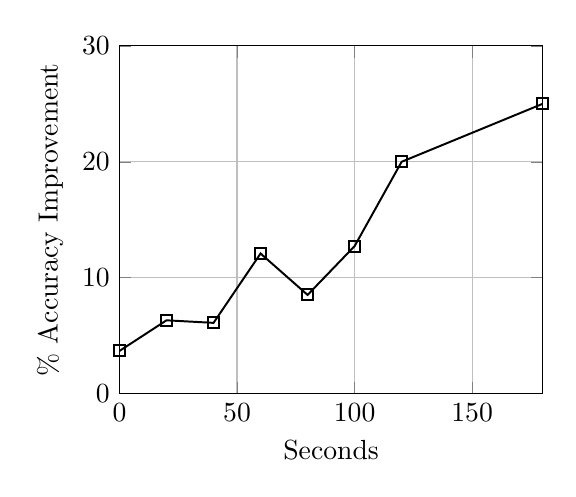
\begin{tikzpicture}
    \begin{axis}[
        % width=12cm, 
        height=6cm,
        xlabel={Seconds},
        ylabel={\% Accuracy Improvement},
        %title={(a) LLaVA Backbone on NeXT-QA},
        xmin=0, xmax=180,
        ymin=0, ymax=30,
        % xtick={5000, 10000, 15000, 20000,25000,30000, 35000},
        % xticklabels={5K, 10K, 15K, 20K, 25K,30K, 35K},
        %ytick={60, 62, 64, 66, 68, 70, 72, 74},
        legend pos=south west,
        grid=both,
        scaled ticks = false,
        scaled x ticks = false,
    ]
\addplot[line width=.25mm, color=black, mark=square, mark size=2pt]
coordinates {
(0, 3.69)
(20, 6.33)
(40, 6.11)
(60, 12.09)
(80, 8.52)
(100, 12.73)
(120, 20)
(180, 25)
};
    \end{axis}
    \end{tikzpicture}
    \caption{LLaVA Backbone on NeXT-QA.}
% \caption{Figure 1}
\end{subfigure}
\hfill
\begin{subfigure}[b]{0.48\textwidth}
    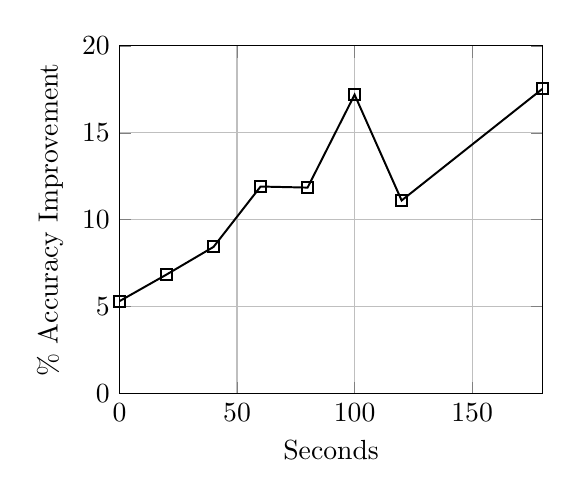
\begin{tikzpicture}
    \begin{axis}[
        % width=12cm, 
        height=6cm,
        xlabel={Seconds},
        ylabel={\% Accuracy Improvement},
        %title={(b) LLaMA Backbone on NeXT-QA},
        xmin=0, xmax=180,
        ymin=0, ymax=20,
        % xtick={5000, 10000, 15000, 20000,25000,30000, 35000},
        % xticklabels={5K, 10K, 15K, 20K, 25K,30K, 35K},
        % ytick={60, 62, 64, 66, 68, 70, 72, 74},
        legend pos=south west,
        grid=both,
        scaled ticks = false,
        scaled x ticks = false,
    ]
    % BIMBA Data

\addplot[line width=.25mm, color=black, mark=square, mark size=2pt]
coordinates {
(0, 5.32)
(20, 6.85)
(40, 8.44)
(60, 11.91)
(80, 11.85)
(100, 17.19)
(120, 11.11)
(180, 17.54)
};
    \end{axis}
    \end{tikzpicture}
    \caption{LLaMA Backbone on NeXT-QA.}
\end{subfigure}
\vspace{-3mm}
\caption{Relative performance improvement of (left) \modelLlava\ over PLLaVA baseline and (right) \modelLlama\ over LLaMA-3.2 (video) baseline for different video durations on NextQA dataset. Our model achieves larger gains as the video length increases.}
\label{fig:performance duration nextqa}
\end{figure*}





In this section, we evaluate the performance of our model on videos of varying lengths from the NextQA~\cite{xiao2021nextqa} dataset, with results presented in \Cref{fig:performance duration nextqa}. \Cref{fig:performance duration nextqa} (left) shows the relative performance improvement over the PLLaVA~\cite{xu2024pllavaparameterfreellava} baseline for different video durations. We observe that as video duration increases, the relative performance improvement over the baseline becomes more pronounced. This demonstrates the effectiveness of our proposed Mamba-based token compression technique compared to pooling-based methods, particularly for long-range videos.


Similarly, the  \Cref{fig:performance duration nextqa} (right) illustrates the relative performance improvement of \modelLlava\ over the LLaMA-3.2 (video) baseline for varying video durations. Here, too, we observe that the relative performance gap widens as video duration increases, showcasing the advantages of our model over the vanilla LLaMA-3.2 (video) baseline, which does not use any compression mechanism.

% \subsection{Comparison with Perceiver Baseline}

% We implement another baseline called Perceiver~\cite{jaegle2021perceiver}, which leverages the widely used Perceiver mechanism to compress the sequence of output tokens generated by the vision encoder before passing them to the LLM. The strategy hinges on using a number of query keys smaller than the number of video input patches processed by the self-attention  operation.  Similar to the other baselines, we experiment with 1, 4, 8, 16, 32, and 64 frames, maintaining the same compression ratio as our model (see ~\Cref{sec:compression} for further details). \Cref{fig:performance1} illustrates the accuracy of LLaVA-based models (top row) and LLaMA-based models (bottom row) on NeXT-QA (left) and EgoSchema (right).
% Our results show that our model consistently outperforms the Perceiver baseline across all scenarios. Furthermore, as the number of frames/tokens increases, the performance gap between our model and the Perceiver baseline widens. This highlights the effectiveness of our Mamba-based token compression technique compared to the Perceiver mechanism, particularly for long-range videos.

\subsection{Computation Cost of \modelLlama}

\begin{figure*}
\centering
\captionsetup[subfigure]{margin={-20mm,-5mm}}
\begin{subfigure}[b]{0.48\textwidth}
    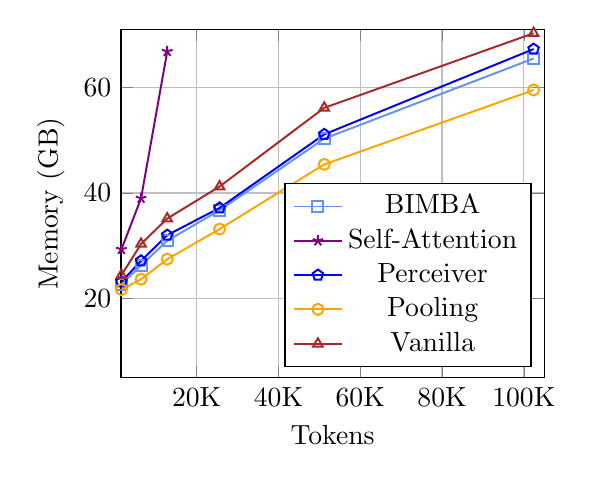
\begin{tikzpicture}
    \begin{axis}[
        % width=12cm, 
        height=6cm,
        xlabel={Tokens},
        ylabel={Memory (GB)},
        %title={(a) Memory Usage of LLaMA-3.2 Backbone},
        xmin=1500, xmax=105000,
        ymin=5, ymax=71,
        %xtick={1600, 6400, 12800, 25600, 51200, 102400},
        % xticklabels={1600, 6400, 12800, 25600, 51200, 102400},
        xtick={20000,40000,60000,80000,100000},
        xticklabels={20K, 40K, 60K, 80K, 100K},
        % ytick={67, 69, 71, 73, 75, 77},
        legend pos=south east,
        grid=both,
        scaled ticks = false,
        scaled x ticks = false,
        % xmode=log,
        % log basis x=1
    ]
    % BIMBA Data
    \addplot[line width=.25mm, color=CornflowerBlue, mark=square, mark size=2pt]
    coordinates {
    (1600, 22.68) (6400, 26.28) (12800, 30.95) (25600, 36.72) (51200, 50.32) (102400, 65.52)
    };
    \addlegendentry{BIMBA}
    
    % Self-Attention Data
    \addplot[line width=.25mm, color=Purple, mark=star, mark size=2pt]
        coordinates {
        (1600, 29.31) (6400, 39.01) (12800, 66.86) 
    };
    \addlegendentry{Self-Attention}

    \addplot[line width=.25mm, color=Blue, mark=pentagon, mark size=2pt]
    coordinates {
    (1600, 23.16) (6400, 27.13) (12800, 32.01) (25600, 37.17) (51200, 51.13) (102400, 67.31)
    };
    \addlegendentry{Perceiver}
    
    % Pooling Data
    \addplot[line width=.25mm, color=Orange, mark=o, mark size=2pt]
    coordinates {
    (1600, 21.67) (6400, 23.65) (12800, 27.45) (25600, 33.16) (51200, 45.44) (102400,59.54)
    };
    \addlegendentry{Pooling}
    \addplot[line width=.25mm, color=Brown, mark=triangle, mark size=2pt]
    coordinates {
    (1600, 24.42) (6400, 30.34) (12800, 35.15) (25600, 41.23) (51200, 56.16) (102400, 70.32)
    };
    \addlegendentry{Vanilla}

    \end{axis}
    \end{tikzpicture}
    \caption{Memory Usage of LLaMA-3.2 Backbone.}
% \caption{Figure 1}
\end{subfigure}
\hfill
\begin{subfigure}[b]{0.48\textwidth}
    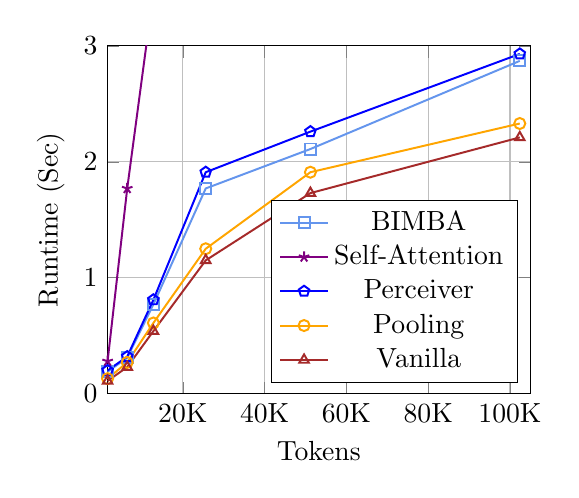
\begin{tikzpicture}
    \begin{axis}[
        % width=12cm, 
        height=6cm,
        xlabel={Tokens},
        ylabel={Runtime (Sec)},
        % title={(b) Runtime of LLaMA-3.2 Backbone},
        xmin=1500, xmax=105000,
        ymin=0, ymax=3,
        %xtick={1600, 6400, 12800, 25600, 51200, 102400},
        % xticklabels={1600, 6400, 12800, 25600, 51200, 102400},
        xtick={20000,40000,60000,80000,100000},
        xticklabels={20K, 40K, 60K, 80K, 100K},
        %ytick={46, 49, 52, 55, 58, 61},
        legend pos=south east,
        grid=both,
        scaled ticks = false,
        scaled x ticks = false,
        % xmode=log,
        % log basis x=1
    ]
    % BIMBA Data
    \addplot[line width=.25mm, color=CornflowerBlue, mark=square, mark size=2pt]
    coordinates {
    (1600, .19) (6400, .31) (12800, .77) (25600, 1.77) (51200, 2.11) (102400, 2.87)
    };
    \addlegendentry{BIMBA}

    
    % Self-Attention Data
    \addplot[line width=.25mm, color=Purple, mark=star, mark size=2pt]
        coordinates {
        (1600, .28) (6400, 1.77) (12800, 3.46)
    };
    \addlegendentry{Self-Attention}

    \addplot[line width=.25mm, color=Blue, mark=pentagon, mark size=2pt]
    coordinates {
    (1600, .2) (6400, .32) (12800, .81) (25600, 1.91) (51200, 2.26) (102400, 2.93)
    };
    \addlegendentry{Perceiver}


    % Pooling Data
    \addplot[line width=.25mm, color=Orange, mark=o, mark size=2pt]
    coordinates {
    (1600, .13) (6400, .27) (12800, .61) (25600, 1.25) (51200, 1.91) (102400, 2.33)
    };
    \addlegendentry{Pooling}


    \addplot[line width=.25mm, color=Brown, mark=triangle, mark size=2pt]
    coordinates {
    (1600, .11) (6400, .23) (12800, .54) (25600, 1.15) (51200, 1.73) (102400, 2.21)
    };
    \addlegendentry{Vanilla}
    
    \end{axis}
    \end{tikzpicture}
    \caption{Runtime of LLaMA-3.2 Backbone.}
    % \caption{Figure 2}
\end{subfigure}
\vspace{-3mm}
\caption{Computation cost of \modelLlama\ and baseline models in terms of memory usage (left) and runtime (right). Self-attention runs out of memory for longer sequences. All other baselines, including our model, maintain low memory and runtime.}
\vspace{-3mm}
\label{fig:computation llama}
\end{figure*}

In this section, we compare the computational cost of our model with other baselines in terms of GPU memory usage (\Cref{fig:computation llama}, left) and runtime (\Cref{fig:computation llama}, right). Our analysis shows that self-attention incurs quadratic costs for both memory and runtime, resulting in out-of-memory errors for inputs longer than 8 frames (12,800 tokens). In contrast, all other methods maintain low memory and runtime costs. Despite having computational efficiency similar to that of the other baselines, our method achieves superior performance, as demonstrated in the previous section. 


\section{Qualitative Results}
\label{sec: qualitative}

Our qualitative results include open-ended video question answering (\Cref{sec:example open-ended}), multiple choice video question answering (\Cref{sec:example multi}), importance of question conditioning (\Cref{sec:example question}), and significance of bidirectional Mamba and interleaved queries (\Cref{sec:example bidirection}).

\subsection{Open-Ended Video Question Answering}
\label{sec:example open-ended}

In \Cref{fig:example open}, we provide examples of our model's performance in open-ended video question answering. The results showcase the model's ability to handle diverse video understanding tasks, including generating detailed descriptions, recognizing objects and interactions, identifying fine-grained activities, and inferring high-level goals. These examples illustrate the model's effectiveness in general-purpose video understanding.

\subsection{Multiple Choice Video Question Answering}
\label{sec:example multi}

We show qualitative examples of video question answering of our model and other baselines on NextQA (\Cref{fig:example nextqa}) and EgoSchema (\Cref{fig:example egoschema}) datasets. Both \modelLlava\ and \modelLlama\ generate the correct answers while other baselines fail, demonstrating the effectiveness of our model for this task. 

\subsection{Importance of Question Conditioning}
\label{sec:example question}

In \Cref{fig:question condition}, we showcase example predictions from our model with and without question-conditioned token selection on the NextQA (\Cref{fig:question condition} (a)) and EgoSchema (\Cref{fig:question condition} (b)) datasets. In both cases, incorporating question tokens into our spatiotemporal token selector enables the model to produce the correct answer. This exhibits the ability of our token selector to leverage question tokens effectively, selecting relevant visual tokens to enhance question-answering performance.


\subsection{Bidirectional Mamba and Interleaved Queries}
\label{sec:example bidirection}

In this section, we visualize the effect of bidirectional Mamba and interleaved queries in \Cref{fig:bidirection and interleaved}. We calculate a response for each frame as follows: first, we take the hidden states of each token after the spatiotemporal token selector and compute a dot product with the query tokens. Then, we apply max pooling to the dot product values of tokens within each frame to obtain a response for that frame. This response value reflects the weight of each frame in the compressed query representations.

\Cref{fig:bidirection and interleaved} (a) shows that using bidirectional scans and interleaved queries enables our model to capture critical information across the entire video and generate the correct answer. In contrast, (b) with bidirectional Mamba and standard queries, the model focuses mainly on the beginning and end of the video, and (c) with unidirectional Mamba and standard queries, the model focuses only on the latter part of the video. Both designs are suboptimal, as they miss critical information and produce incorrect answers.

% \begin{figure*}[t]
\footnotesize
\centering
\vspace{-10mm}
\captionsetup[subfigure]{margin={-20mm,-5mm}}
\begin{subfigure}[b]{0.48\textwidth}
    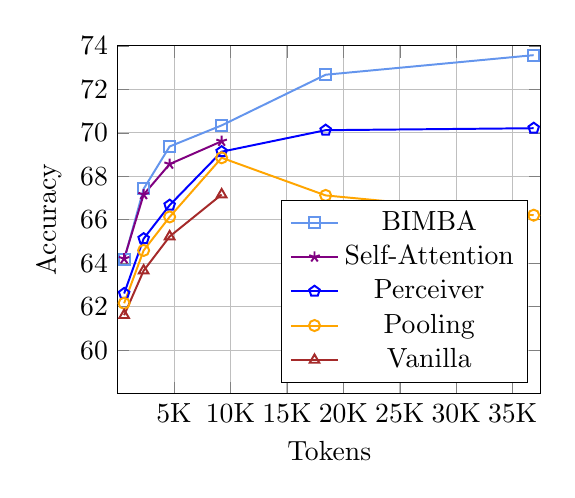
\begin{tikzpicture}
    \begin{axis}[
        % width=12cm, 
        height=6cm,
        xlabel={Tokens},
        ylabel={Accuracy},
        %title={(a) LLaVA Backbone on NeXT-QA},
        xmin=0, xmax=37500,
        ymin=58, ymax=74,
        %xtick={576, 2304, 4608, 9216, 18432, 36864},
        % xticklabels={576, 2304, 4608, 9216, 18432, 36864},
        xtick={5000, 10000, 15000, 20000,25000,30000, 35000},
        xticklabels={5K, 10K, 15K, 20K, 25K,30K, 35K},
        ytick={60, 62, 64, 66, 68, 70, 72, 74},
        legend pos=south east,
        grid=both,
        scaled ticks = false,
        scaled x ticks = false,
        % xmode=log,
        % log basis x=1
    ]
    % BIMBA Data
    \addplot[line width=.25mm, color=CornflowerBlue, mark=square, mark size=2pt]
    coordinates {
    (576, 64.16) (2304, 67.42) (4608, 69.37) (9216, 70.34) (18432, 72.67) (36864, 73.57)
    };
    \addlegendentry{BIMBA}
    
    % Self-Attention Data
    \addplot[line width=.25mm, color=Purple, mark=star, mark size=2pt]
        coordinates {
        (576, 64.21) (2304, 67.16) (4608, 68.56) (9216, 69.61)
    };
    \addlegendentry{Self-Attention}

    \addplot[line width=.25mm, color=Blue, mark=pentagon, mark size=2pt]
    coordinates {
    (576, 62.61) (2304, 65.13) (4608, 66.67) (9216, 69.13) (18432, 70.12) (36864, 70.21)
    };
    \addlegendentry{Perceiver}
    
    % Pooling Data
    \addplot[line width=.25mm, color=Orange, mark=o, mark size=2pt]
    coordinates {
    (576, 62.16) (2304, 64.59) (4608, 66.13) (9216, 68.85) (18432, 67.12) (36864, 66.21)
    };
    \addlegendentry{Pooling}

    \addplot[line width=.25mm, color=Brown, mark=triangle, mark size=2pt]
    coordinates {
    (576, 61.61) (2304, 63.66) (4608, 65.23) (9216, 67.16) 
    };
    \addlegendentry{Vanilla}
    \end{axis}
    \end{tikzpicture}
    \vspace{-1mm}
    \caption{NExT-QA performance of models based on LLaVA.}
    \vspace{1mm}
\end{subfigure}
\hfill
\begin{subfigure}[b]{0.48\textwidth}
    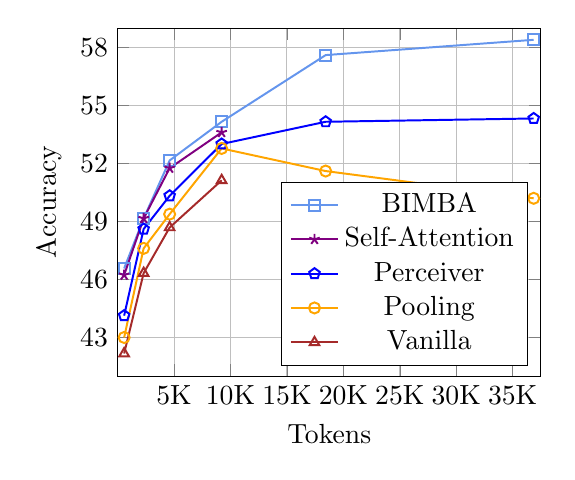
\begin{tikzpicture}
    \begin{axis}[
        % width=12cm, height=8cm,
        %height=7cm,
        height=6cm,
        xlabel={Tokens},
        ylabel={Accuracy},
        %title={(b) LLaVA Backbone on EgoSchema},
        xmin=0, xmax=37500,
        ymin=41, ymax=59,
        %xtick={576, 2304, 4608, 9216, 18432, 36864},
        % xticklabels={576, 2304, 4608, 9216, 18432, 36864},
        xtick={5000, 10000, 15000, 20000,25000,30000, 35000},
        xticklabels={5K, 10K, 15K, 20K, 25K,30K, 35K},
        ytick={43, 46, 49, 52, 55, 58, 61},
        legend pos=south east,
        grid=both,
        scaled ticks = false,
        scaled x ticks = false,
        % xmode=log,
        % log basis x=1
    ]
    % BIMBA Data
    \addplot[line width=.25mm, color=CornflowerBlue, mark=square, mark size=2pt]
    coordinates {
    (576, 46.57) (2304, 49.16) (4608, 52.16) (9216, 54.16) (18432, 57.61) (36864, 58.40)
    };
    \addlegendentry{BIMBA}

    % Self-Attention Data
    \addplot[line width=.25mm, color=Purple, mark=star, mark size=2pt]
        coordinates {
        (576, 46.23) (2304, 49.16) (4608, 51.76) (9216, 53.61)
    };
    \addlegendentry{Self-Attention}

    \addplot[line width=.25mm, color=Blue, mark=pentagon, mark size=2pt]
    coordinates {
    (576, 44.13) (2304, 48.61) (4608, 50.33) (9216, 53.01) (18432, 54.16) (36864, 54.33)
    };
    \addlegendentry{Perceiver}

    % Pooling Data
    \addplot[line width=.25mm, color=Orange, mark=o, mark size=2pt]
    coordinates {
    (576, 43.00) (2304, 47.61) (4608, 49.38) (9216, 52.78) (18432, 51.61) (36864, 50.20)
    };
    \addlegendentry{Pooling}

    \addplot[line width=.25mm, color=Brown, mark=triangle, mark size=2pt]
    coordinates {
    (576, 42.17) (2304, 46.33) (4608, 48.69) (9216, 51.13) 
    };
    \addlegendentry{Vanilla}
    \end{axis}
    \end{tikzpicture}
    \vspace{-1mm}
    \caption{EgoSchema performance of models based on LLaVA.}
    \vspace{1mm}
\end{subfigure}
\begin{subfigure}[b]{0.48\textwidth}
    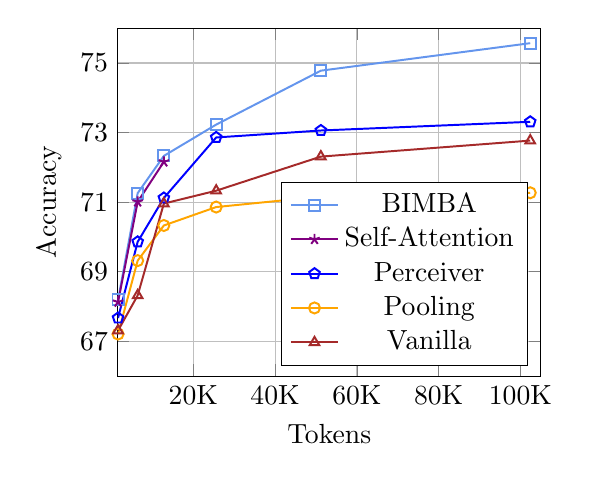
\begin{tikzpicture}
    \begin{axis}[
        % width=12cm, height=8cm,
        %height=7cm,
        height=6cm,
        xlabel={Tokens},
        ylabel={Accuracy},
        %title={(a) LLaMA Backbone on NeXT-QA},
        xmin=1500, xmax=105000,
        ymin=66, ymax=76,
        %xtick={1600, 6400, 12800, 25600, 51200, 102400},
        % xticklabels={1600, 6400, 12800, 25600, 51200, 102400},
        xtick={20000,40000,60000,80000,100000},
        xticklabels={20K, 40K, 60K, 80K, 100K},
        ytick={67, 69, 71, 73, 75, 77},
        legend pos=south east,
        grid=both,
        scaled ticks = false,
        scaled x ticks = false,
        % xmode=log,
        % log basis x=1
    ]
    % BIMBA Data
    \addplot[line width=.25mm, color=CornflowerBlue, mark=square, mark size=2pt]
    coordinates {
    (1600, 68.19) (6400, 71.26) (12800, 72.33) (25600, 73.23) (51200, 74.78) (102400, 75.57)
    };
    \addlegendentry{BIMBA}
    
    % Self-Attention Data
    \addplot[line width=.25mm, color=Purple, mark=star, mark size=2pt]
        coordinates {
        (1600, 68.13) (6400, 71.01) (12800, 72.16) 
    };
    \addlegendentry{Self-Attention}

    \addplot[line width=.25mm, color=Blue, mark=pentagon, mark size=2pt]
    coordinates {
    (1600, 67.67) (6400, 69.86) (12800, 71.12) (25600, 72.86) (51200, 73.06) (102400, 73.31)
    };
    \addlegendentry{Perceiver}
    
    % Pooling Data
    \addplot[line width=.25mm, color=Orange, mark=o, mark size=2pt]
    coordinates {
    (1600, 67.21) (6400, 69.32) (12800, 70.33) (25600, 70.86) (51200, 71.16) (102400, 71.27)
    };
    \addlegendentry{Pooling}
    \addplot[line width=.25mm, color=Brown, mark=triangle, mark size=2pt]
    coordinates {
    (1600, 67.31) (6400, 68.32) (12800, 70.96) (25600, 71.33) (51200, 72.31) (102400, 72.77)
    };
    \addlegendentry{Vanilla}
    \end{axis}
    \end{tikzpicture}
    \caption{NExT-QA performance of models based on LLaMA.}
% \caption{Figure 1}
\end{subfigure}
\hfill
\begin{subfigure}[b]{0.48\textwidth}
    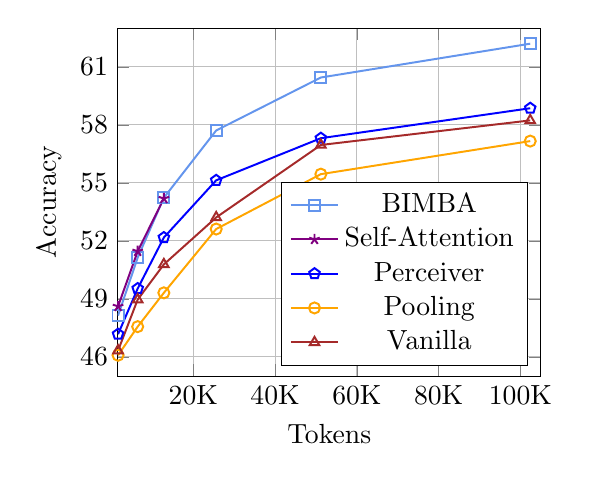
\begin{tikzpicture}
    \begin{axis}[
        % width=12cm, height=8cm,
        height=6cm,
        xlabel={Tokens},
        ylabel={Accuracy},
        %title={(b) LLaMA Backbone on EgoSchema},
        xmin=1500, xmax=105000,
        ymin=45, ymax=63,
        %xtick={1600, 6400, 12800, 25600, 51200, 102400},
        % xticklabels={1600, 6400, 12800, 25600, 51200, 102400},
        xtick={20000,40000,60000,80000,100000},
        xticklabels={20K, 40K, 60K, 80K, 100K},
        ytick={46, 49, 52, 55, 58, 61},
        legend pos=south east,
        grid=both,
        scaled ticks = false,
        scaled x ticks = false,
        % xmode=log,
        % log basis x=1
    ]
    % BIMBA Data
    \addplot[line width=.25mm, color=CornflowerBlue, mark=square, mark size=2pt]
    coordinates {
    (1600, 48.13) (6400, 51.13) (12800, 54.23) (25600, 57.71) (51200, 60.45) (102400, 62.20)
    };
    \addlegendentry{BIMBA}
    
    % Self-Attention Data
    \addplot[line width=.25mm, color=Purple, mark=star, mark size=2pt]
        coordinates {
        (1600, 48.61) (6400, 51.46) (12800, 54.19)
    };
    \addlegendentry{Self-Attention}

    \addplot[line width=.25mm, color=Blue, mark=pentagon, mark size=2pt]
    coordinates {
    (1600, 47.17) (6400, 49.53) (12800, 52.17) (25600, 55.13) (51200, 57.31) (102400, 58.86)
    };
    \addlegendentry{Perceiver}

    % Pooling Data
    \addplot[line width=.25mm, color=Orange, mark=o, mark size=2pt]
    coordinates {
    (1600, 46.08) (6400, 47.56) (12800, 49.31) (25600, 52.61) (51200, 55.45) (102400, 57.16)
    };
    \addlegendentry{Pooling}

    \addplot[line width=.25mm, color=Brown, mark=triangle, mark size=2pt]
    coordinates {
    (1600, 46.32) (6400, 48.96) (12800, 50.78) (25600, 53.21) (51200, 56.96) (102400, 58.23)
    };
    \addlegendentry{Vanilla}
    \end{axis}
    \end{tikzpicture}
    \caption{EgoSchema performance of models based on the LLaMA.}
\end{subfigure}
\vspace{-2mm}
\caption{\small{Accuracy achieved by \model\ and baseline models on NeXT-QA (left) and EgoSchema (right) as a function of the number of input tokens for models based on LLaVA (top row) and LLaMA (bottom row). \model\ achieves the highest accuracy for all sequence lengths, and the difference with other baselines increases as we 
increase the number of input tokens. Self-attention cannot be applied to long sequences as it causes GPU out-of-memory issues once the number of tokens becomes too large.}}
\vspace{-5mm}
\label{fig:performance1}
\end{figure*}

% \LT{add arrow and ``out of memory''}

\begin{figure*}[t]
\begin{subfigure}[b]{1\textwidth}
    \centering
    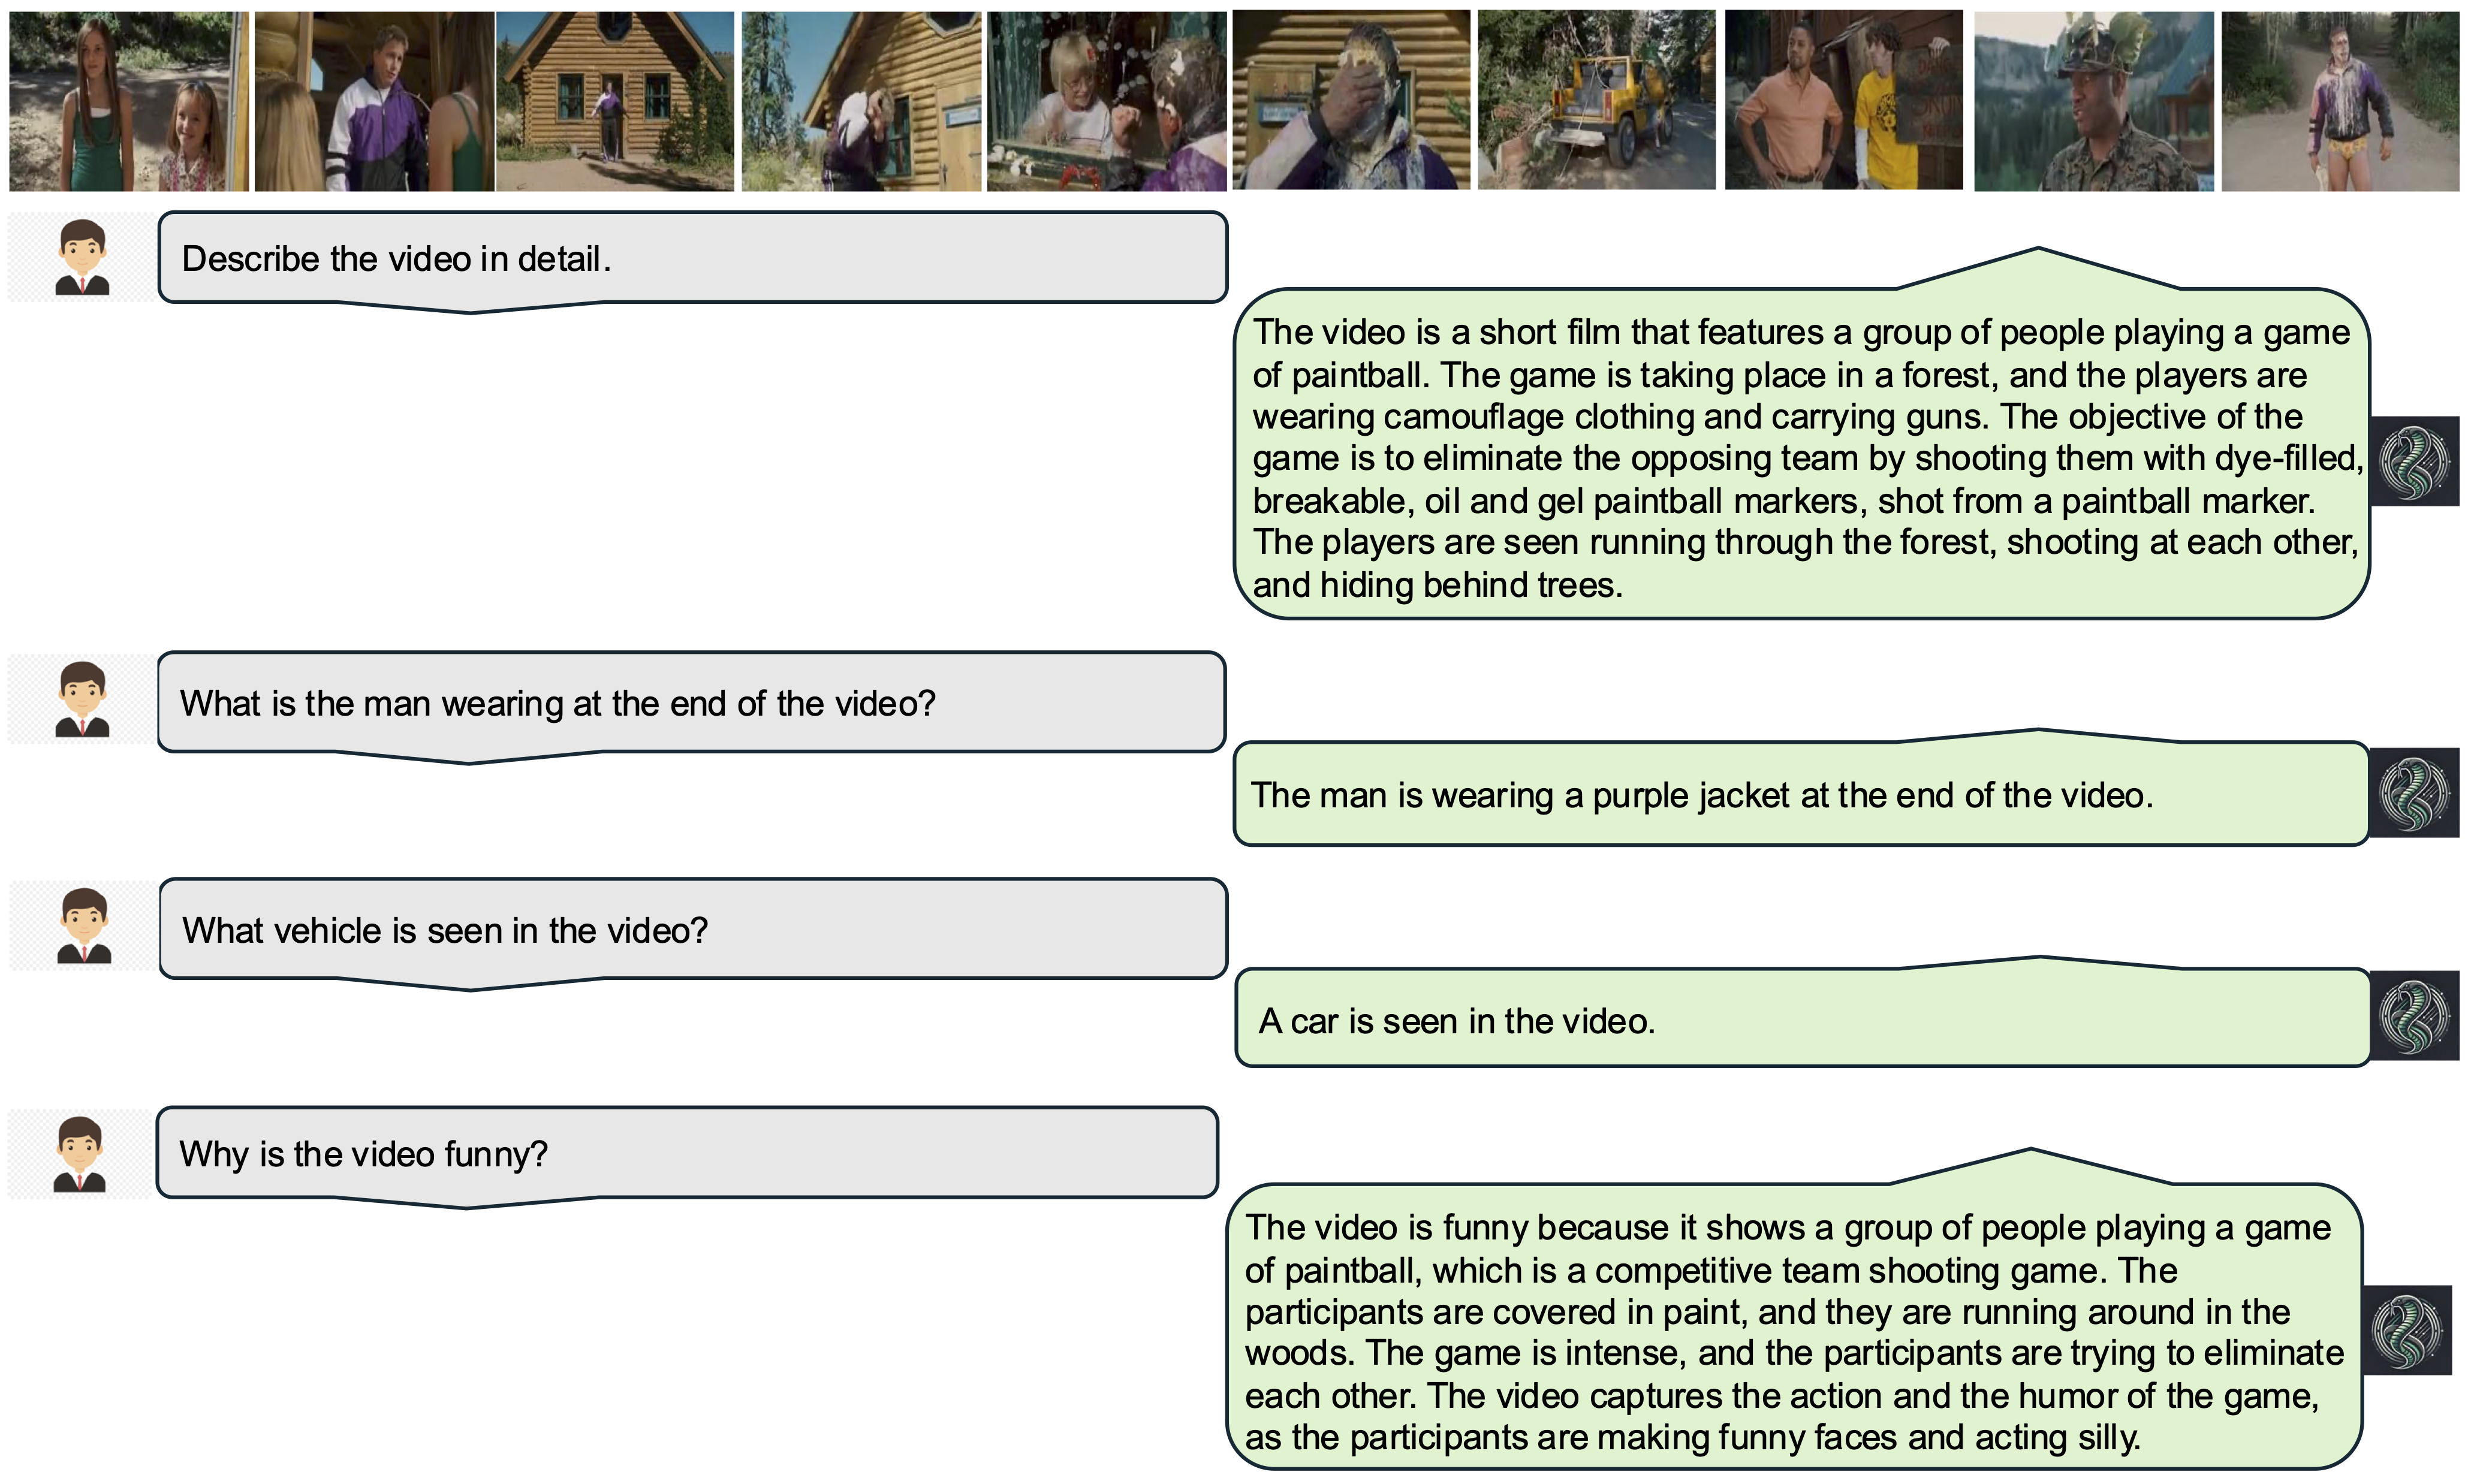
\includegraphics[width=\textwidth]{figures/conversation_movie.png}
    \caption{Example 1 of open-ended video question answering.}
\end{subfigure}
\begin{subfigure}[b]{1\textwidth}
    \centering
    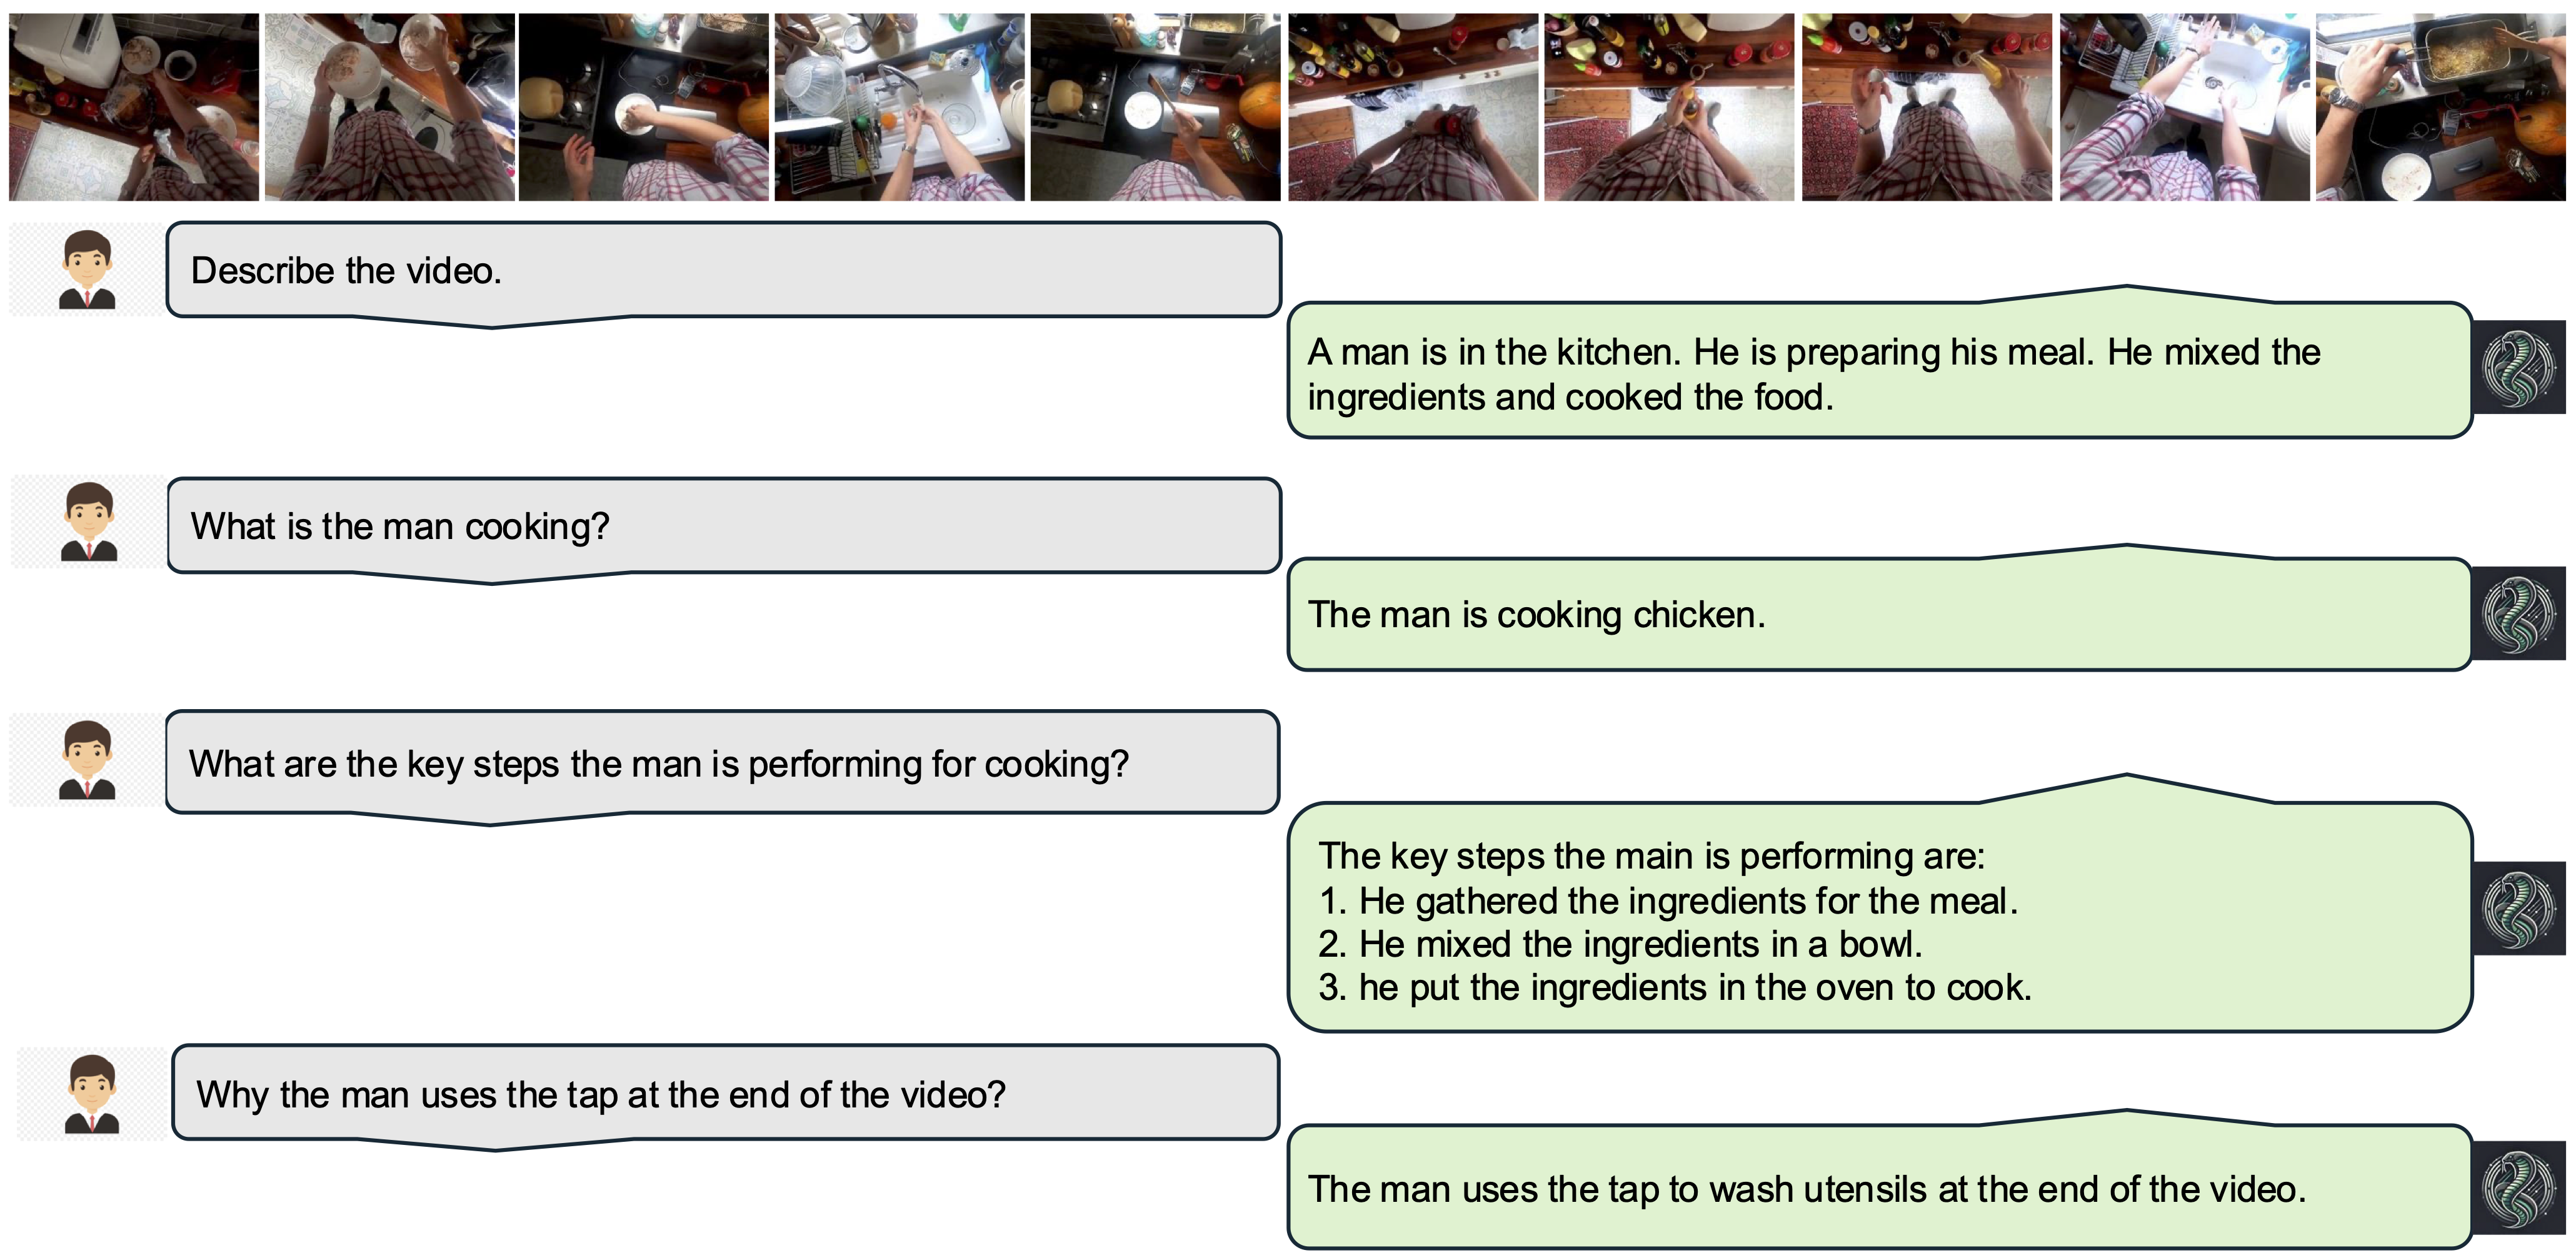
\includegraphics[width=\textwidth]{figures/conversation_egoschema.png}
    \caption{Example 2 of open-ended video question answering.}
\end{subfigure}
\caption{Qualitative Results on Open-Ended Video Question Answering. Our model demonstrates the ability to answer a wide range of questions about videos, including detailed descriptions, high-level goals, and fine-grained activities.}
\label{fig:example open}
\end{figure*}

% \begin{figure*}[t]
%     \centering
%     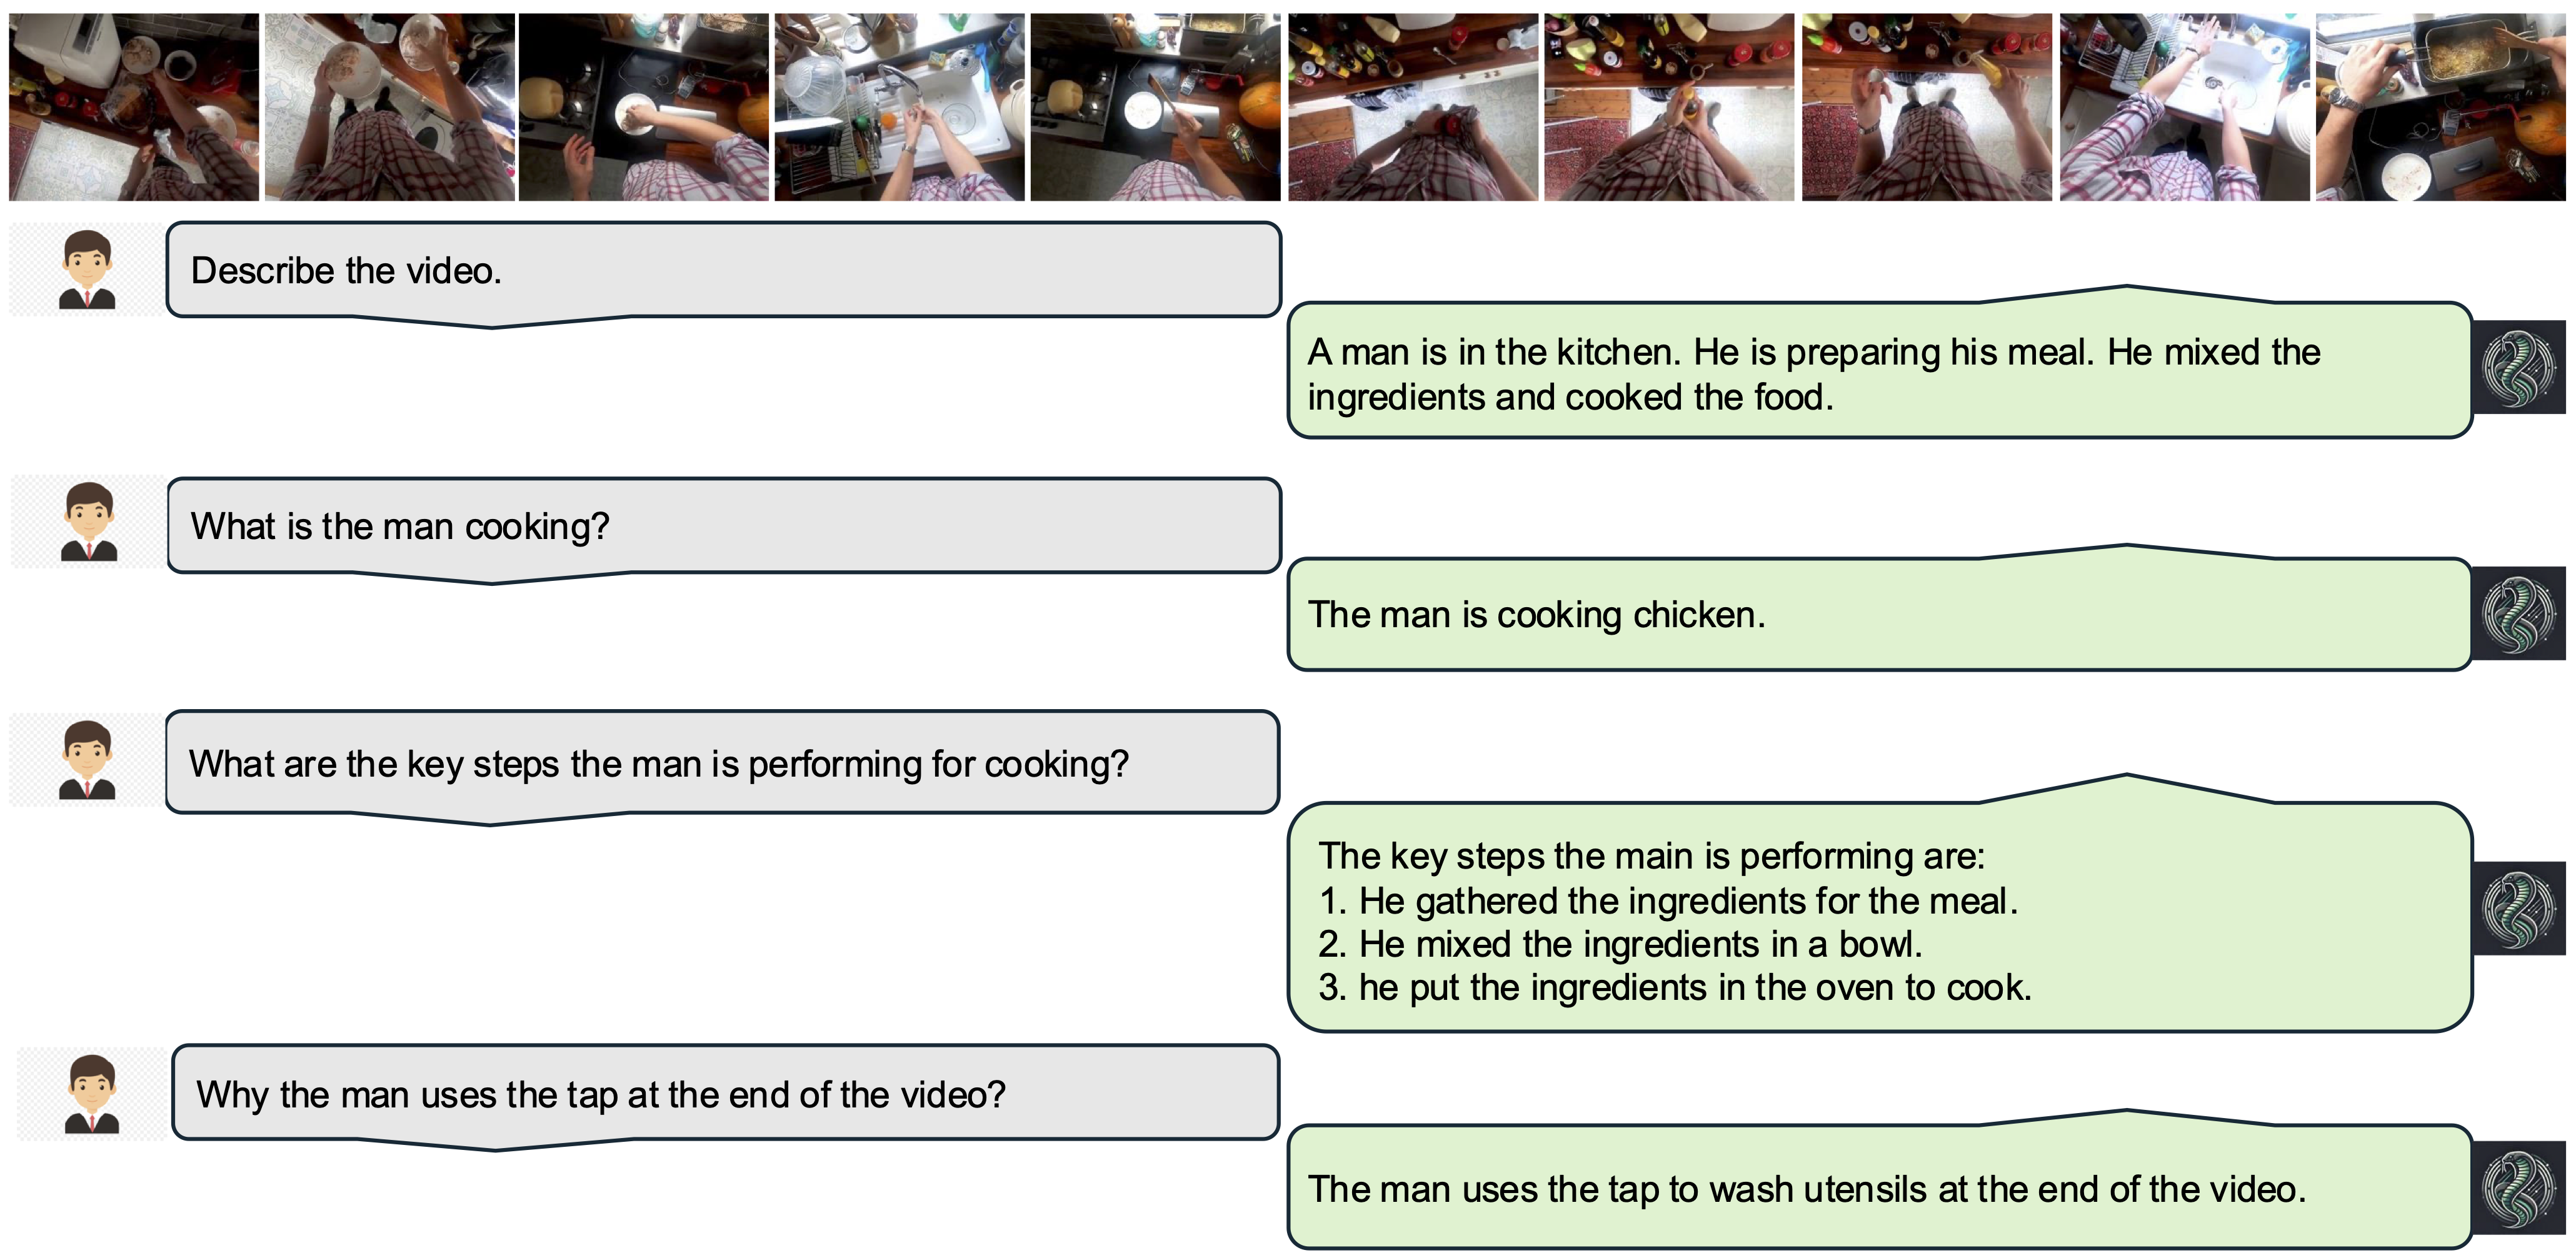
\includegraphics[width=\textwidth]{figures/conversation_egoschema.png}
%     \caption{Qualitative Results.}
% \label{fig:example nextqa}
% \end{figure*}

\begin{figure*}[t]
    \centering
    \includegraphics[width=\textwidth]{figures/example_nextqa_no_face.png}
    \caption{Qualitative Results on NextQA. Our model generates the correct answer while both PLLaVA and LLaMA-3.2 (video) baselines fail.}
\label{fig:example nextqa}
\end{figure*}

\begin{figure*}[t]
    \centering
    \includegraphics[width=\textwidth]{figures/example_egoschema.png}
    \caption{Qualitative Results on EgoSchema. Our model generates the correct answer while both PLLaVA and LLaMA-3.2 (video) baselines fail.}
\label{fig:example egoschema}
\end{figure*}


\begin{figure*}[t]
    \centering
    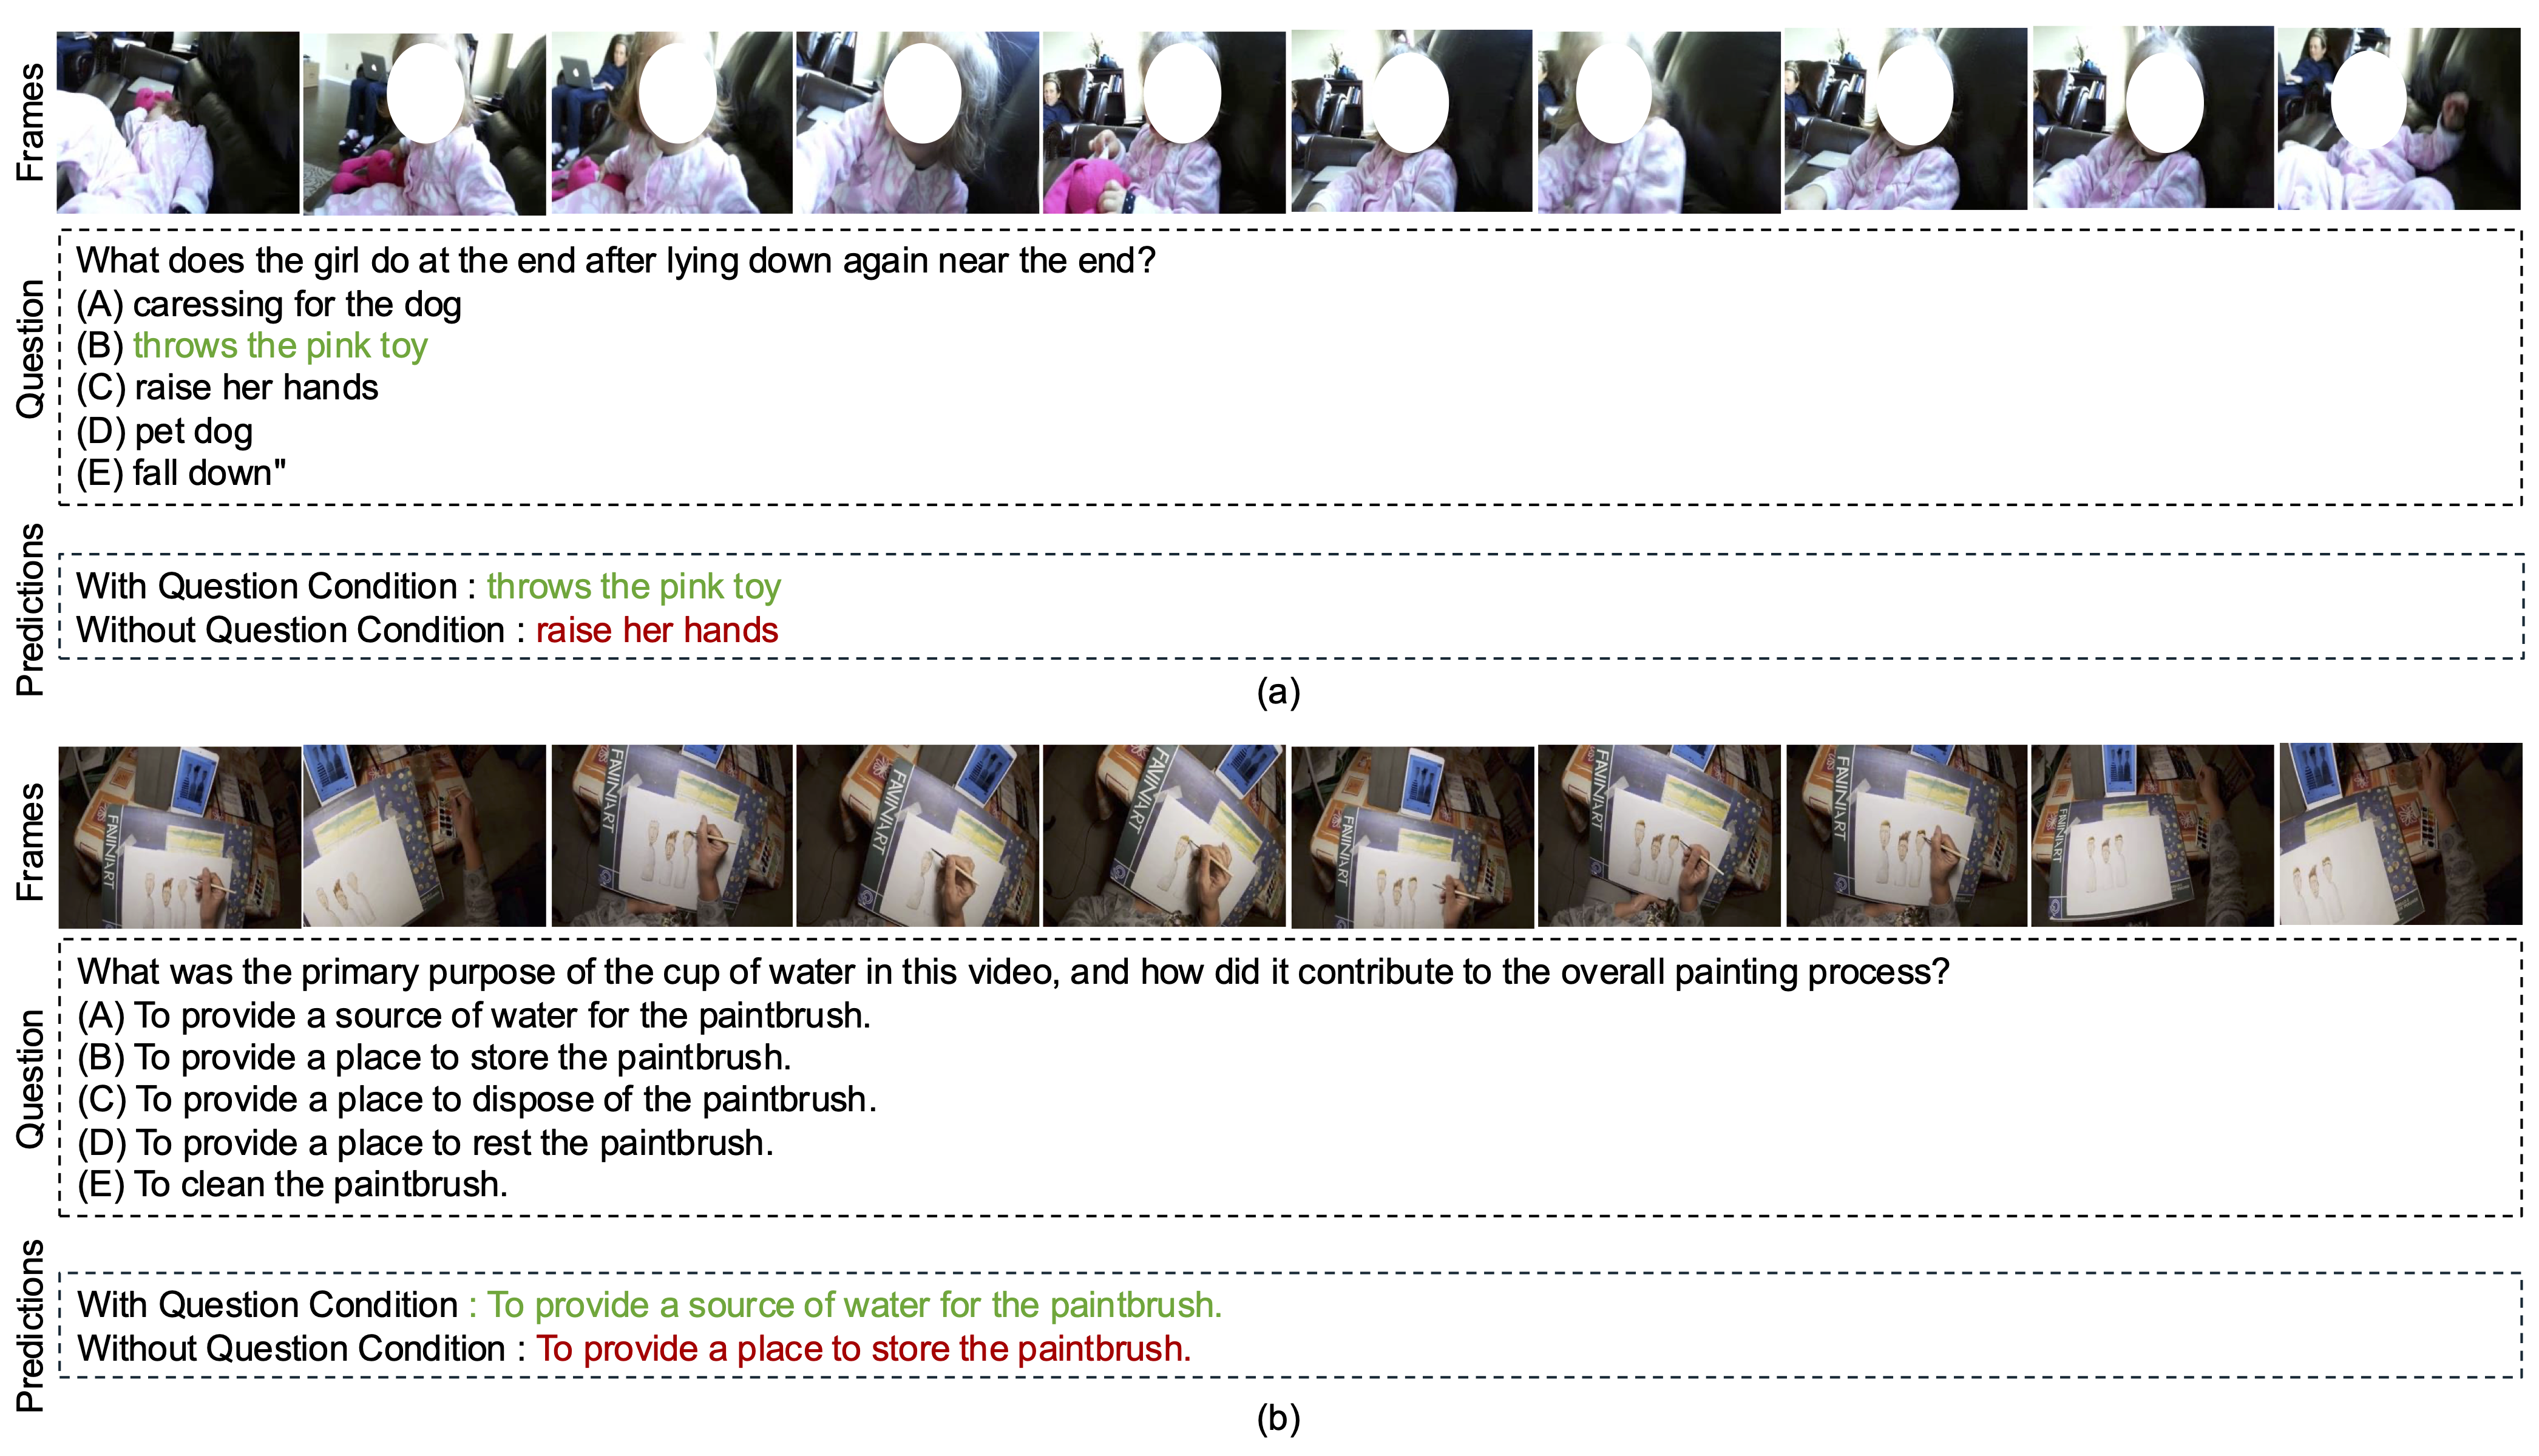
\includegraphics[width=\textwidth]{figures/question_condition_no_face.png}
    \caption{Qualitative Results on Question Conditioned Token Selection on (a) NextQA and (b) EgoSchema datasets. Incorporating question tokens into our spatiotemporal token selector leads to the correct answer in both examples. Using the information from the questions allows our spatiotemporal selection module to focus on the most relevant video parts for answering the question.}
\label{fig:question condition}
\end{figure*}

\begin{figure*}[t]
    \centering
    \includegraphics[width=\textwidth]{figures/mamba_bidir_inter_ego.png}
    \caption{Visualization of Bidirectional Mamba and Interleave Queries. Utilizing bidirectional Mamba and interleaved queries leads to the correct answer, while the unidirectional Mamba and standard queries fail.}
\label{fig:bidirection and interleaved}
\end{figure*}
